\usetikzlibrary{decorations.markings}

\begin{center}
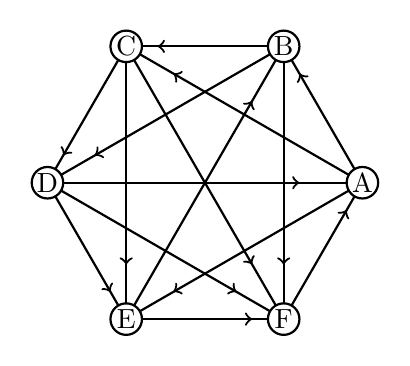
\begin{tikzpicture}[scale=2]
\coordinate (A) at (2.00000,1.00000);
\coordinate (B) at (1.50000,1.86603);
\coordinate (C) at (0.50000,1.86603);
\coordinate (D) at (0.00000,1.00000);
\coordinate (E) at (0.50000,0.13397);
\coordinate (F) at (1.50000,0.13397);

\begin{scope}[thick,decoration={
    markings,
    mark=at position 0.8 with {\arrow{>}}}
    ] 
    \draw[thick, postaction={decorate}] (A) -- (B);
    \draw[thick, postaction={decorate}] (A) -- (C);
    \draw[thick, postaction={decorate}] (D) -- (A);
    \draw[thick, postaction={decorate}] (A) -- (E);
    \draw[thick, postaction={decorate}] (F) -- (A);
    \draw[thick, postaction={decorate}] (B) -- (C);
    \draw[thick, postaction={decorate}] (B) -- (D);
    \draw[thick, postaction={decorate}] (E) -- (B);
    \draw[thick, postaction={decorate}] (B) -- (F);
    \draw[thick, postaction={decorate}] (C) -- (D);
    \draw[thick, postaction={decorate}] (C) -- (E);
    \draw[thick, postaction={decorate}] (C) -- (F);
    \draw[thick, postaction={decorate}] (D) -- (E);
    \draw[thick, postaction={decorate}] (D) -- (F);
    \draw[thick, postaction={decorate}] (E) -- (F);
\end{scope}
\draw[thick, fill=white] (A) circle (0.1) node {A};
\draw[thick, fill=white] (B) circle (0.1) node {B};
\draw[thick, fill=white] (C) circle (0.1) node {C};
\draw[thick, fill=white] (D) circle (0.1) node {D};
\draw[thick, fill=white] (E) circle (0.1) node {E};
\draw[thick, fill=white] (F) circle (0.1) node {F};
\end{tikzpicture}
\end{center}
